\documentclass{article}
\usepackage[utf8]{inputenc}
\title{MATH 20C Notes - Week Six}
\author{C-Rin}
\date{October 2019}

\usepackage{natbib}
\usepackage{graphicx}
\usepackage{gensymb}
\usepackage{amsmath}
\usepackage{amssymb}
\usepackage{wrapfig}
\usepackage{diffcoeff}
\usepackage{microtype}

\graphicspath{ {./images/} }

\begin{document}

\maketitle

\section*{Introduction}
Deep 

\begin{figure}[h!]
\centering
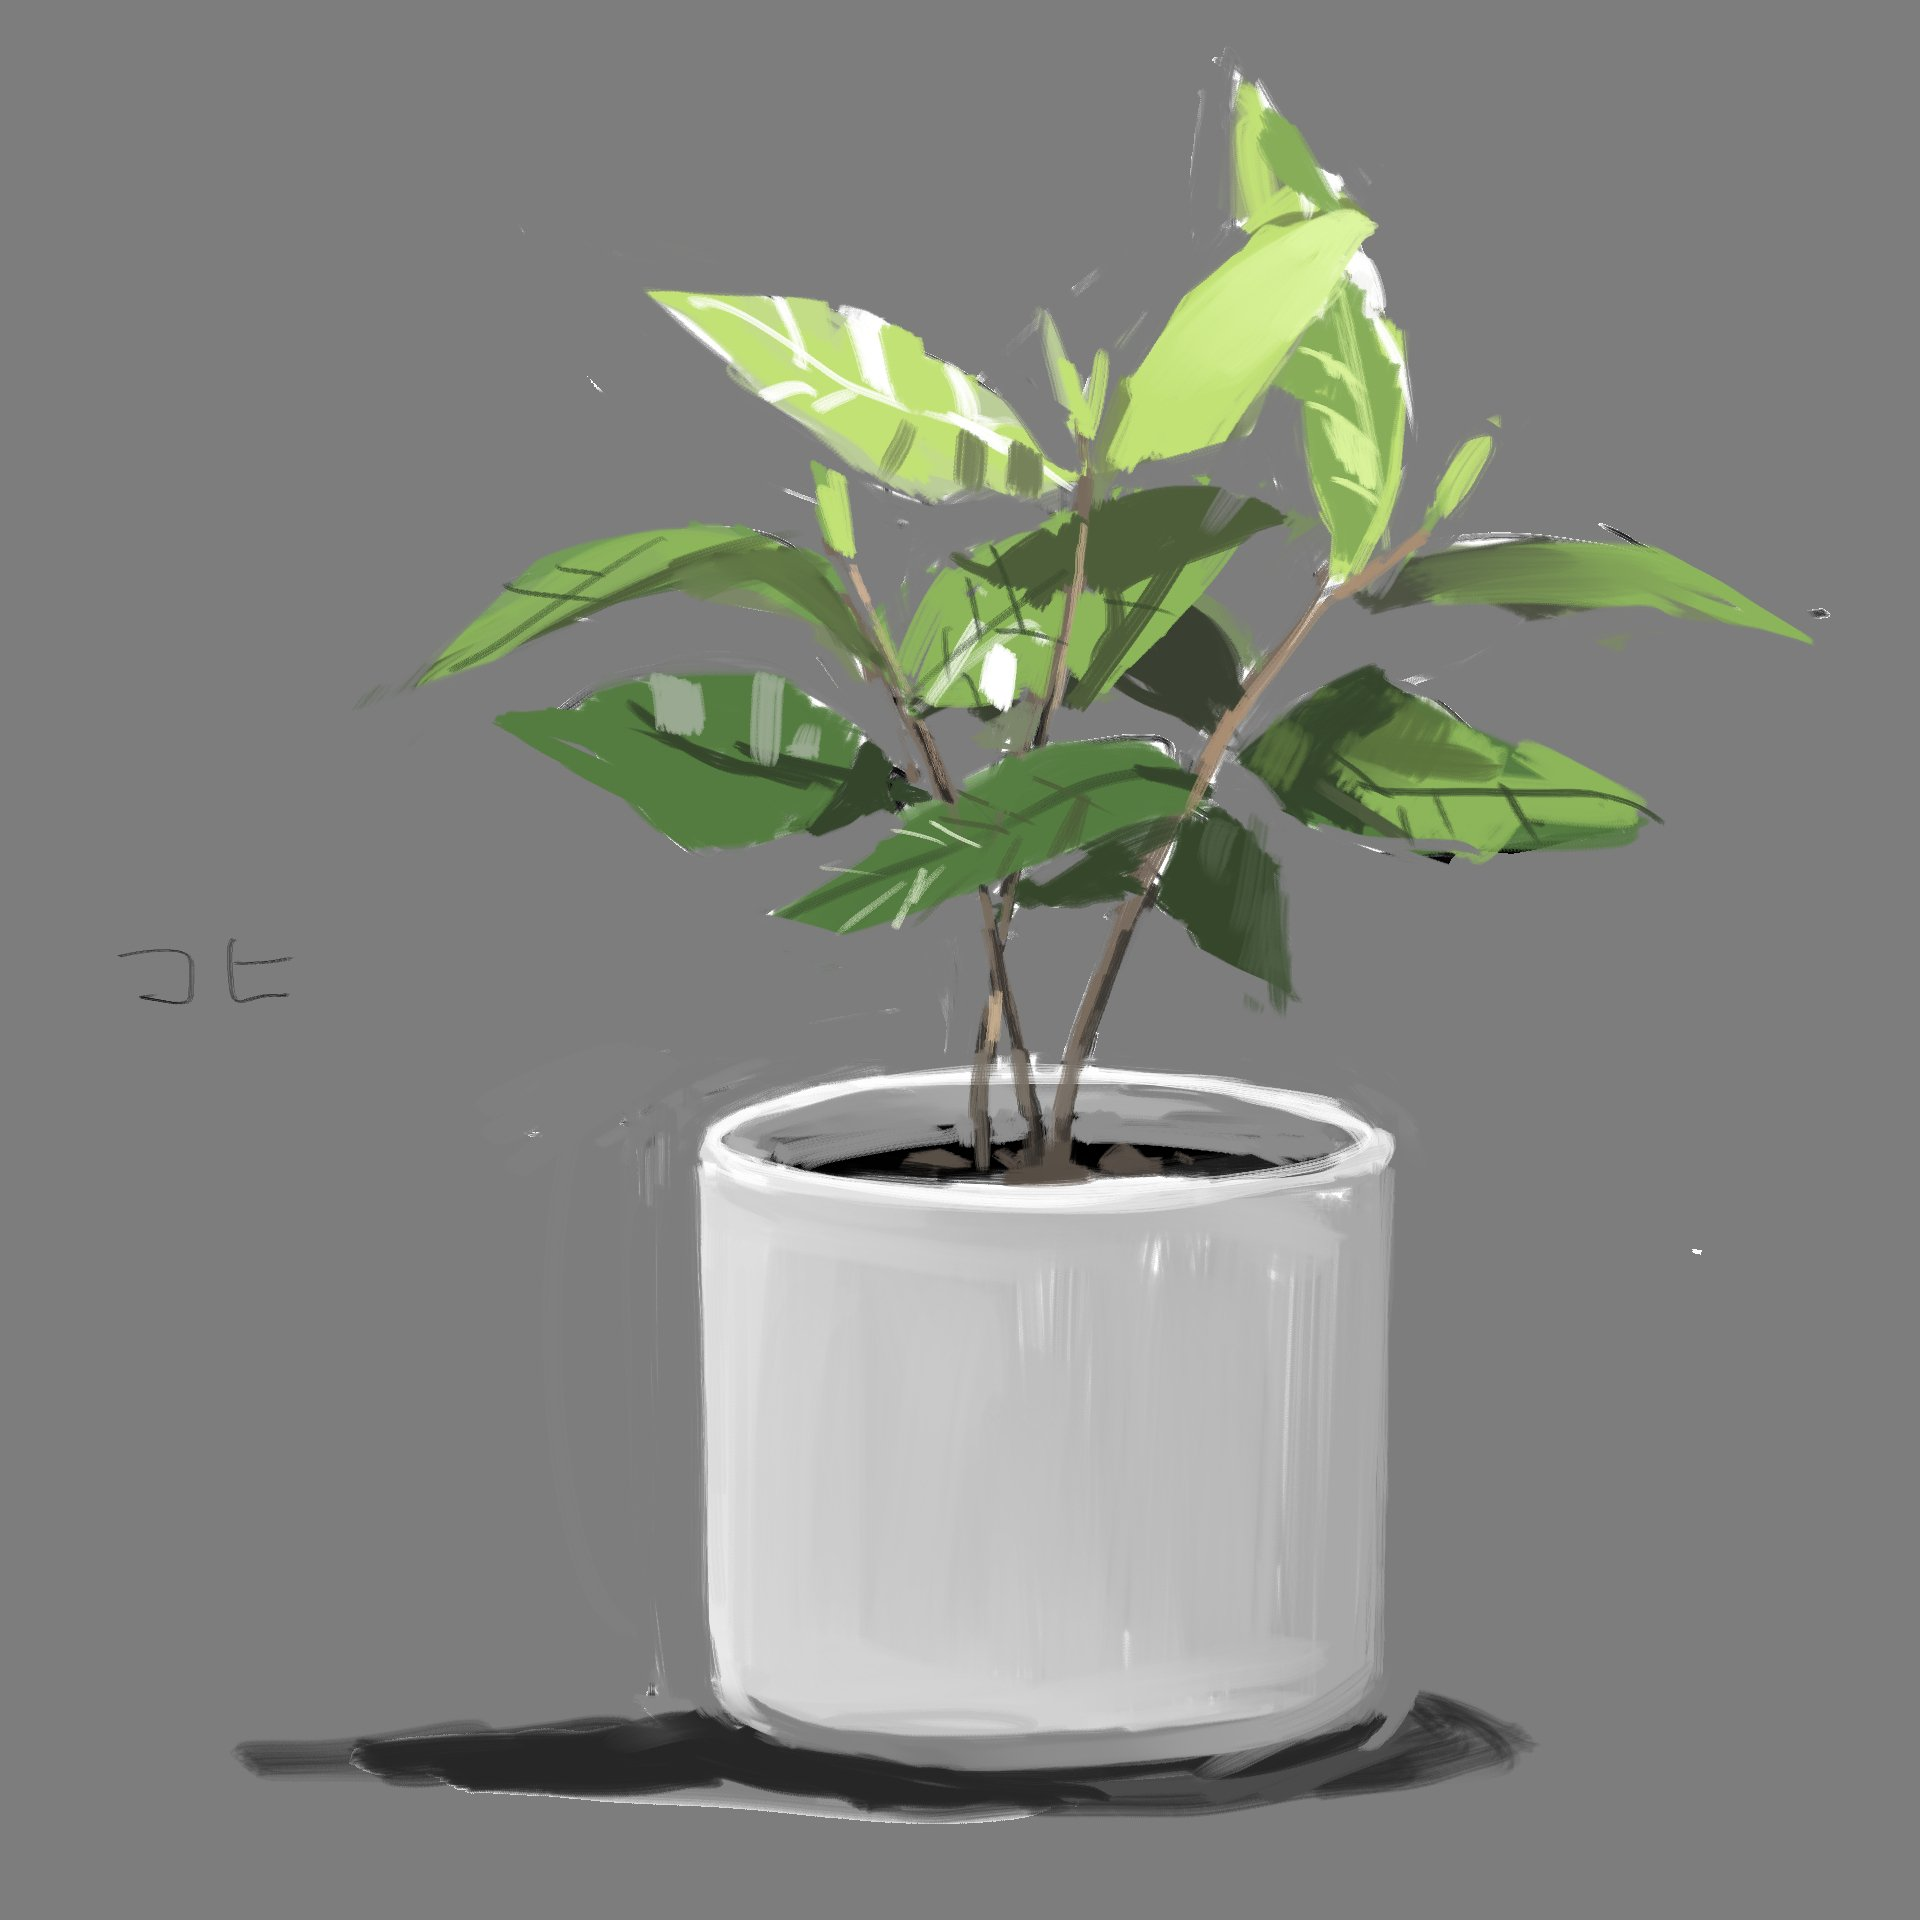
\includegraphics[scale=0.1]{plant.jpg}
\caption{A plant (unspecified species)}
\end{figure}


\newpage
\section{Extrema of Real Valued Functions}
\[f:U\rightarrow\mathbb{R} \qquad  U\overbrace{\subseteq}^{\mbox{subset}} \mathbb{R}^2 \qquad U\mbox{ is an "open subset"}\]

An open subset is a subset value for any point $x\in U$ \\
In an open subset, you can move an arbitrarily small amount in any direction while staying in the subset.
\begin{figure}[h!]
    \centering
    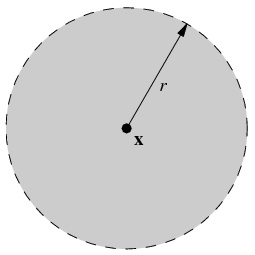
\includegraphics[scale = .5]{OpenDisk.jpg}
    \caption{An open disk with $U=\{\vec{v}\in \mathbb{R}^2\Big| ||\vec{v}||<1\}$}
    \label{}
\end{figure}

\subsection*{Maximum and Minimum Extrema}
Q: What is the definition of a maximum (or minimum) of $f$?

A: A point $\vec{v}\in U$ is a maximum if $f(\vec{v})$ is greater or equal to $f(\vec{w})$ for any $\vec{w}\in U$ (Similarly defined for a minimum)

\subsection*{Definitions}
\begin{enumerate}
    \item An open neighborhood of a point $x\in U$ is an open set $v\in U$ which contains $x$.
    \item A point $x\in U$ is a local max (respectively a local minimum) if there is an open neighborhood of $x$ where $x$ is a maximum (respectively a minimum)
    \item A $x\in U$ is a \underline{critical point} if either
    \begin{enumerate}
        \item $f$ is not differentiable at $x$\\[5pt]
        \textbf{OR}
        \item $Df(x)=0$
    \end{enumerate}
    \item A critical point which is not a local maximum or minimum is a saddle point
\end{enumerate}

\subsection*{Theorem}
Let $f: U\rightarrow\mathbb{R}$ and $U\subseteq\mathbb{R}^n$ be a differentiable function.

If $\vec{v}\in U$ and $\vec{v}$ is a local extremum, then $Df(\vec{v})=0$ (i.e. $\vec{v}$ is a critical point).


\subsection*{Example}

$f:\mathbb{R}^2\rightarrow\mathbb{R}\qquad f(x,y)=\log(x^2+y^2+1)$\\[6pt]
Find all the critical points.

\[
\ooalign{
  $\overbrace{\mathbb{R}^2\;\;\rightarrow\;\;\mathbb{R}^3}^{g(x)=x^2+y^2+1}\rightarrow\;\;\mathbb{R}$\cr
  $\phantom{\mathbb{R}^2\;\;\rightarrow\;\;{}} {\underbrace{\phantom{\mathbb{R}^3\rightarrow\;\;\mathbb{R}}}_{h(z)=\log(z)}} $\cr
}
\]

\[Df(x,y)=Dh(x^2+y^2+1)\cdot Dg(x,y)\]
\[=\begin{bmatrix}
    \frac{1}{x^2+y^2+1}
\end{bmatrix}\cdot\begin{bmatrix}
    2x&2y
\end{bmatrix}\]
\[=\begin{bmatrix}
    \frac{2x}{x^2+y^2+1}&\frac{2y}{x^2+y^2+1}
\end{bmatrix}=\begin{bmatrix}
    0&0
\end{bmatrix}\]

\[(x,y)=(0,0)\]

\subsection*{Example}
Find all the critical points in $\mathbb{R}^2$ for $f(x,y)=2(x^2+y^2)\cdot e^{-x^2-y^2}$
\begin{wrapfigure}{r}{0.2\textwidth}
    \begin{center}
      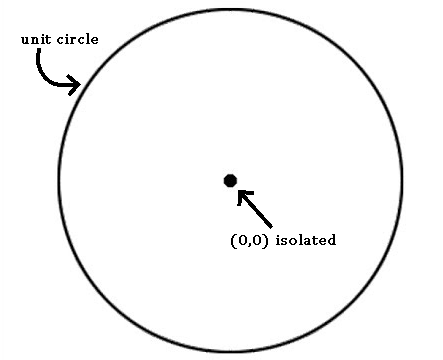
\includegraphics[width=0.40\textwidth]{unitCircle.png}
    \end{center}
  \end{wrapfigure}
\[f(x,y)=2(x^2+y^2)\cdot e^{-(x^2+y^2)}\qquad h(z)=x^2+y^2\qquad g(z)=2z\cdot e^{-z}\]
\[Dg(z)=2ze^[-z]+2z(-e^{-z})=2e^{-z}-2ze^{-z}=[2e^{-z}(1-z)]\]
\[=[2e^{-x^2-y^2}(1-x^2-y^2)]\]\\[6pt]
\[Dg\circ h=\begin{bmatrix}
    2e^{-x^2-y^2}(1-x^2-y^2)
\end{bmatrix}\begin{bmatrix}
    2x&2y
\end{bmatrix}\]
\[=\begin{bmatrix}
    4xe^{-x^2-y^2}(1-x^2-y^2)&4ye^{-x^2-y^2}(1-x^2-y^2)
\end{bmatrix}\]

\[\begin{bmatrix}
    4xe^{-x^2-y^2}(1-x^2-y^2)&4ye^{-x^2-y^2}(1-x^2-y^2)
\end{bmatrix}=\begin{bmatrix}
    0&0
\end{bmatrix}\]

\[(x,y)=(0,0),(1,0),(0,1), \mbox{ and all the values on the unit circle}\]
\newpage
\section{2nd Derivative Test for Extrema}
\subsection*{Theorem}
Let $f(x,y)$ be a $c^2$ function and suppose
\begin{enumerate}
    \item The derivative $Df(x_o,y_o)=0$
    \item $\frac{\partial^2 f}{\partial x^2}(x_o,y_o)>0$
    \item $D=(\frac{\partial^2 f}{\partial x^2})(\frac{\partial^2 f}{\partial y^2})-(\frac{\partial^2 f}{\partial x \partial y})^{2}>0$
\end{enumerate}
Then $(x_o,y_o)$ is an isolated local minimum. If $\frac{\partial^2 f}{\partial x^2}(\vec{v} <0)$, and 1. and 3. hold, then $\vec{v}$ is a local maximum.

\subsection*{Remarks}
\begin{enumerate}
    \item D is the determinant of the following 2x2 matrix, known as a Hessian Matrix.
    \item If $\vec{v}$ is a critical point, but $D<0$ at $\vec{v}$, then $\vec{v}$ is a saddle point.
\end{enumerate}
\begin{wrapfigure}{r}{0.2\textwidth}
    \begin{center}
      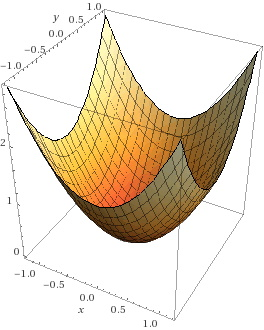
\includegraphics[width=0.40\textwidth]{graph1.jpg}
    \end{center}
  \end{wrapfigure}
\[\underbrace{\begin{bmatrix}
    \frac{\partial^2 f}{\partial x^2}& \frac{\partial^2 f}{\partial x \partial y}\\
    \frac{\partial^2 f}{\partial y \partial x}& \frac{\partial^2 f}{\partial y^2}
\end{bmatrix}}_{\mbox{A Hessian Matrix}}\]\\

A saddle point is a point on the surface of the graph of a function where the slopes (derivatives) in orthogonal directions are all zero (a critical point), but which is not a local extremum of the function.

\subsection*{Example}

Find the critical points of $x^2+y^2=f(x,y)$
\subsubsection*{Critical Points}

We need to find $\frac{\partial^2 f}{\partial y^2},\frac{\partial^2 f}{\partial x^2},\frac{\partial^2 f}{\partial x \partial y}$
\[\nabla f(x,y)=\begin{bmatrix}
    2x&2y
\end{bmatrix}\qquad \frac{\partial^2 f}{\partial x^2}=2>0\]
\[\frac{\partial^2 f}{\partial y^2}=2\qquad \frac{\partial^2 f}{\partial x \partial y}=0\]

This is a local minimum due to the second derivative test.

\subsection*{Exercise}
Find the critical points of $f(x,y)=x^{5}y+xy^3+xy$ and determine if they are local extrema or saddle points.

\[Df(x,y)=\begin{bmatrix}
    5x^4y+y^3+y& x^5+3xy^2+x
\end{bmatrix}\]
\[\mbox{Critical points }(x,y)=(0,0)\]
\[D=\frac{\partial^2 f}{\partial x^2}\cdot \frac{\partial^2 f}{\partial y^2}-(\frac{\partial^2 f}{\partial x \partial y})^2\]

\section{Closed Sets}
A closed set is a set which contains all of its boundary points. 

A closed unit disc would be an example with the bounds $\{\vec{v}\in \mathbb{R}^2\Big| ||\vec{v}||\leq 1 \}$

A nonexample would be an open unit disc, which does not contain any of its boundary points. 

A subset of $\mathbb{R}^2$ is bounded if it is contained in some arbitrarily "large enough" circle.

\subsection*{Example}
Every Square is bounded.
\begin{figure}[h!]
    \centering
    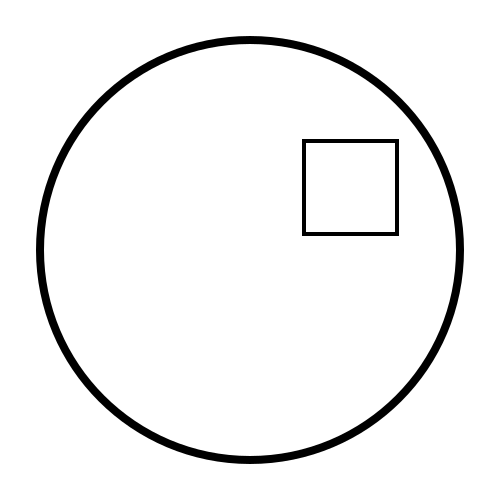
\includegraphics[scale =.15]{squareInCircle.png}
    \caption{Every square has a circle that can make it bounded}
    \label{}
\end{figure}

\subsection*{Nonexample}
The x-axis is always unbounded, where at some point it is not in the circle.
\begin{figure}[h!]
    \centering
    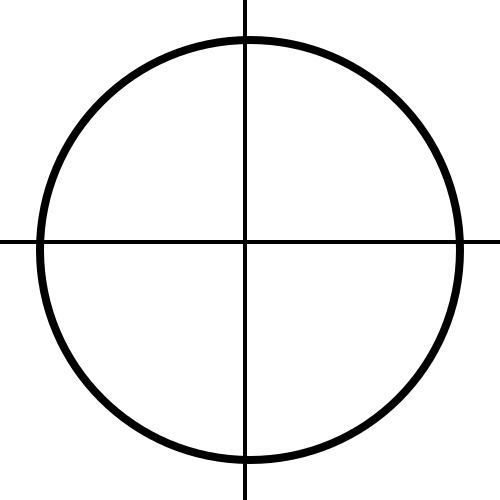
\includegraphics[scale=.15]{lineInCircle.png}
    \caption{At some point, the line passes through the circle, no matter how big the circle is.}
    \label{}
\end{figure}
\subsection*{Theorem}
If you have any two sets $f:z\rightarrow\mathbb{R}$ is a continuous function and $z\subseteq\mathbb{R}^2$ is closed and bounded, then the function has a maximum and a minimum.

\begin{figure}[h!]
    \centering
    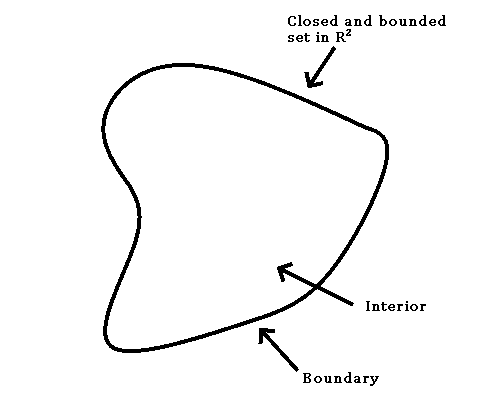
\includegraphics[scale=.5]{closedAndBounded.png}
    \caption{A closed and bounded set in $\mathbb{R}^2$}
    \label{}
\end{figure}
The set of interior points is an open set.

\section{The Optimization Method}

\begin{enumerate}
    \item Find all the critical points on the interior
    \item Use the path and try to find all the critical points of $f(\vec{g}(t))$
    \item Compare the values of the critical points (i.e. plug them in)
\end{enumerate}

\subsection*{Example}
Find the maximum/minimum $f(x,y)=x^2+y^2-x-y+1$ on the closed unit disk.

To do this, we need to parameterize the boundary.

\begin{wrapfigure}{r}{0.2\textwidth}
    \begin{center}
      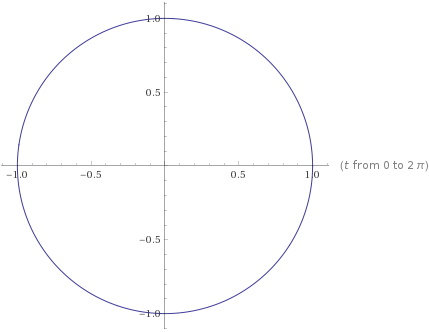
\includegraphics[width=0.40\textwidth]{wolframUnitCircle.jpg}
    \end{center}
\end{wrapfigure}

\[Df(x,y) = \begin{bmatrix}
    2x-1&2y-1
\end{bmatrix}=\begin{bmatrix}
    0&0
\end{bmatrix}\qquad (x,y)=(1/2,1/2)\]
\[f(\vec{g}(t))=\overbrace{\cos^{2}(t)+\sin^{2}(t)}^{1}-\cos(t)-\sin(t)+1\]
\[=2-\cos(t)-sin(t)\]

What is the domain of $t$?

In this situation, $[0,2\pi]$ works.
\[f^\prime (\vec{g}(t))=\sin(t)-\cos(t)=0\mbox{  when $\sin(t)=\cos(t)$}\]
\[t=\frac{\pi}{4},\frac{5\pi}{4}\mbox{ (and possibly $0$ and $2\pi$)}\]
\[f(1/2,1/2)=\frac{1}{2}\qquad f(\vec{g}(0))=1\]

\[f(\vec{g}(\frac{\pi}{4}))=\frac{1}{2}+\frac{1}{2}-\frac{\sqrt{2}}{2}-\frac{\sqrt{2}}{2}=1-\sqrt{2}\qquad f(\vec{g}(\frac{5\pi}{4}))=2+\sqrt{2}\]

\section{Constrained Extrema and \\Lagrange Multipliers}
\subsection*{Optimizing functions and level sets \\
(A.K.A) The Lagrange Error}

\subsection*{Theorem}
$U\subseteq\mathbb{R}^n$ is an open set, and $f:U\rightarrow\mathbb{R}$ and $g:U\rightarrow\mathbb{R}$ are two differentiable functions.


Let S be a level set of $g$ on level $c$.\\

If $f$ has a local maximum or minimum on S at a point $\vec{v}$ in S and $\nabla g(\vec{v})\neq 0$, then there exists a real number $\lambda$ such that 
\[\nabla f(\vec{v})=\lambda \nabla g(\vec{v})\]

\subsection*{Example}
\[\underbrace{S\subseteq\mathbb{R}^2}_{S\leftarrow y=x+1}\qquad f(x,y)=x^2+y^2\]
Find the local extrema of $f$ on $S$.




\end{document}